%!TEX root=demo-paper.tex

\section{Introduction}
\label{sec:introduction}


Data analysts must sift through very large volumes of data 
to identify trends, insights, or anomalies. 
Given the scale of data, and the relative ease and 
intuitiveness of examining data visually,
analysts often use visualizations as a tool to identify
these trends, insights, and anomalies.
However, selecting the ``right'' visualization often 
remains a laborious and time-consuming task. 

We illustrate the data analysis process using an example. 
Consider a dataset containing sales records for a nation-wide
chain of stores.
Let's say the store's data analyst is interested
in examining how the newly-introduced heating device, the ``Laserwave
Oven'', has been doing over the past year.
The results of this analysis will inform business decisions
for the chain, including marketing strategies, and the introduction of a similar
``Saberwave Oven''.

The analysis workflow proceeds as follows:
(1) The analyst poses a query to select the subset of data that he are
interested in exploring.
For instance, for the example above, he may issue the query:
\noindent $${\tt \ Q \ \ = \ \ SELECT \ * \ FROM \ \  Sales \ \ WHERE \ \
Product=``Laserwave''} $$ \noindent Notice that the results for this query may
have (say) several million records each with several dozen attributes.
Thus, directly perusing the query result is simply infeasible.
(2) Next, the analyst studies various properties of the selected data by
constructing diverse views or visualizations from the data. In this particular
scenario, the analyst may want to study total sales by store, quantity in stock
by region, or average profits by month. To construct these views, the analyst
can use operations such as binning, grouping, and aggregation, and then generate
visualizations from the view. For example, to generate the view `total sales by
store', the analyst would group each sales record based on the store where the
sale took place and add up the sale amounts per store. This operation can easily
be expressed as the familiar aggregate-plus-group-by query:
\noindent
\begin{align*}
& \tt Q' = SELECT \ \ SUM(amount) \ \ FROM \ \  Sales \ \ WHERE \\
& \tt Product=``Laserwave" \ \ GROUP  \ \ BY \ \ store
\end{align*}
The result of the above query is a two-column table that can then be visualized
as a bar-chart. Table \ref{tab:staplerX} and Figure
\ref{fig:staplerX} respectively show an example of the results of this view and
the associated visualization.
To explore the query results from different perspectives, the analyst generates
a large number of views (and visualizations) of the form described above.
(3) The analyst then manually examines each view and decides
which ones are ``interesting''. This is the critical and time-consuming step.
Naturally, what makes a view interesting depends on the 
application semantics and the trend we are comparing against.
For instance, the view of Laserwave sales by store, as shown in Figure
\ref{fig:staplerX}, may be interesting if the overall sales of all products show
the {\it opposite} trend (e.g. Figure \ref{fig:staplerX-a}). However, the same
view may be uninteresting if the sales of all products follow a similar trend (Figure \ref{fig:staplerX-b}).
Thus, we posit that  a view is {\em potentially ``interesting'' if it shows 
a trend in the subset of data selected by the analyst
(i.e., Laserwave product-related data)
that deviates from the equivalent trend in the overall dataset}.
Of course, the analyst must decide if this deviation 
is truly an insight for this application.
(4) Once the analyst has identified interesting views, the analyst may
then either share these views with others, further interact with
the displayed views (e.g. by drilling down or rolling up), or
start afresh with a new query.


Of the four steps in the workflow described above, the 
ones that are especially repetitive and tedious are steps (2) and (3),
where the analyst generates a large number of candidate views, and examines each
of them in turn. The goal of our system, \SeeDB, is to automate these
labor-intensive steps of the workflow. Given a query $Q$ indicating the subset
of data that the analyst is interested in, \SeeDB\ automatically {\em identifies and highlights to the analyst the most
interesting views of the query results using methods based on
deviation}. Specifically, \SeeDB\ explores the space of all possible views and
measures how much each view deviates from the corresponding view on the
entire underlying dataset (e.g. Figure~\ref{fig:staplerX} vs.
Figures~\ref{fig:staplerX-a} or \ref{fig:staplerX-b}.) By generating and
scoring potential views automatically, \SeeDB\ effectively eliminates
steps (2) and (3) that the analyst currently performs. Instead, once \SeeDB\
recommends interesting views, the analyst can evaluate this small
subset of views using domain knowledge and limit further
exploration to these views.  

We described our vision for \SeeDB, along with the associated research
challenges in a companion vision paper~\cite{DBLP:conf/vldb/Parameswaran2013}.
In this demonstration proposal, we present our first \SeeDB\ prototype
addressing some of the challenges listed in that vision paper.
In particular, our current prototype of \SeeDB\ is built as a ``wrapper'' that
can be overlaid on any relational database system. Given any query, \SeeDB\
leverages special optimization algorithms and the underlying DBMS to generate
and recommend interesting visualizations. To do so efficiently and accurately,
we must address the following challenges:
(a) We must determine metrics that accurately measure the ``deviation'' of a
view with respect to the equivalent view on the entire database (e.g.,
Figure~\ref{fig:staplerX} vs.~\ref{fig:staplerX-a}), while simultaneouly
ensuring that \SeeDB\ is not tied to any particular metric(s); (b) We must
intelligently explore the space of candidate views. Since the number of
candidate views (or visualizations) increases as the square of the number of
attributes in a table (we will demonstrate this in subsequent sections),
generating and evaluating all views, even for a moderately sized dataset (e.g.
1M rows, 100 attributes), can be prohibitively expensive;
(c) While executing queries corresponding to different views, we must share
computation as much as possible. Queries to compute views and their
deviation are highly similar and therefore
independent execution is expensive and wasteful; (d) Since
analysis must happen in real-time, we must trade-off accuracy
of visualizations or estimation of ``interestingness'' for reduced latency.
Section~\ref{sec:system_architecture} describes how we address these challenges.



% of Step 1), we demonstrate that we can automatically explore various views of
% that data, evaluate each one for ``interesting''-ness and only surface the most
% promising views to the analyst. 



% In this demo, we demonstrate a system called \SeeDB\
% \cite{DBLP:conf/vldb/Parameswaran2013} that automates the labor-intensive parts
% of the aforementioned data analysis process by automatically identifying and
% producing high-quality views for any input query. Specifically, given a query
% $Q$ posed by the user, \SeeDB\ explores all possible views of $Q$, determines
% the ``interesting''-ness of each of the views based on deviation and returns to
% the user the set of views that it deems the most interesting. The user can then
% limit his analysis to this high-quality set of views.

% In the process of automatically producing an interesting set of views for any
% query, \SeeDB\ must address a few challenges: (a) the size of the space of
% potential views increases as the square of the number of attributes in a table,
% and even for a moderately sized table (e.g. 1M rows, 100 attributes) generating
% all views is prohibitively expensive; as a result, \SeeDB\ must intelligently
% explore this space; (b) computing each view and its utility independently is
% expensive and wasteful, and hence \SeeDB\ must share computation between
% queries; and (c) since visual analysis must happen in real-time, \SeeDB\ must
% tradeoff accuracy of views for reduced latency. In Section
% \ref{sec:system_architecture}, we describe how \SeeDB\ addresses these
% challenges.


% Consider a medical researcher studying the cost of care for cancer patients. Her
% research involves the analysis of a set of 1M electronic medical records (EMRs).
% To analyze this data, the researcher identifies patients that cost
% significantly more than the average: specifically, she selects patients whose
% cost of care is greater than the average cost by two standard deviations. In
% terms of SQL, she runs the following query: \\

% \noindent 
% \begin{small}
% \begin{verbatim}
% Q = SELECT * FROM Patients where total_cost - 
% (SELECT AVG(total_cost) from Patients) as avg_cost
% > 2 * (SELECT STDDEV(total_cost) from Patients);
% \end{verbatim}
% \end{small}

% Once she has identified these patients, she must study various aspects of their
% care to determine the reason why the patients have large cost of care. For
% instance, she may study length of treatment, survival rate, severity of disease
% etc. For each of these parameters, she is interested in determining how the
% group of patients with high cost of care are different from the overall group of
% patients. As a result, she may construct various views of the data that
% compare various metrics between the high cost patients and the overall patient
% population. For instance, she may compare the distribution of length of
% treatment for the two populations, the average severity of the disease
% etc. Since there are a large number of metrics that may be responsible for high
% cost of care, the analyst must construct, visualize and examine a large number
% of views to identify interesting trends. For more than 5 metrics, this process
% quickly becomes tedious and time-consuming. We can significantly simplify and
% speed up the analysis process if we can automate the creation and evaluation of
% views.


\begin{figure}
\CenterFloatBoxes
\begin{floatrow}
\ttabbox{%
  \small
  \begin{tabular}{cc} \hline
  Store & Total Sales (\$) \\ \hline
  Cambridge, MA & 180.55 \\ \hline
  Seattle, WA &  145.50\\ \hline
  New York, NY & 122.00 \\ \hline
  San Francisco, CA & 90.13 \\ \hline
  \end{tabular}
}{%
  \caption{Data: Total Sales by Store for Laserwave}\label{tab:staplerX}%
}
\killfloatstyle
\ffigbox{%
  \hbox{\resizebox{2cm}{2cm}{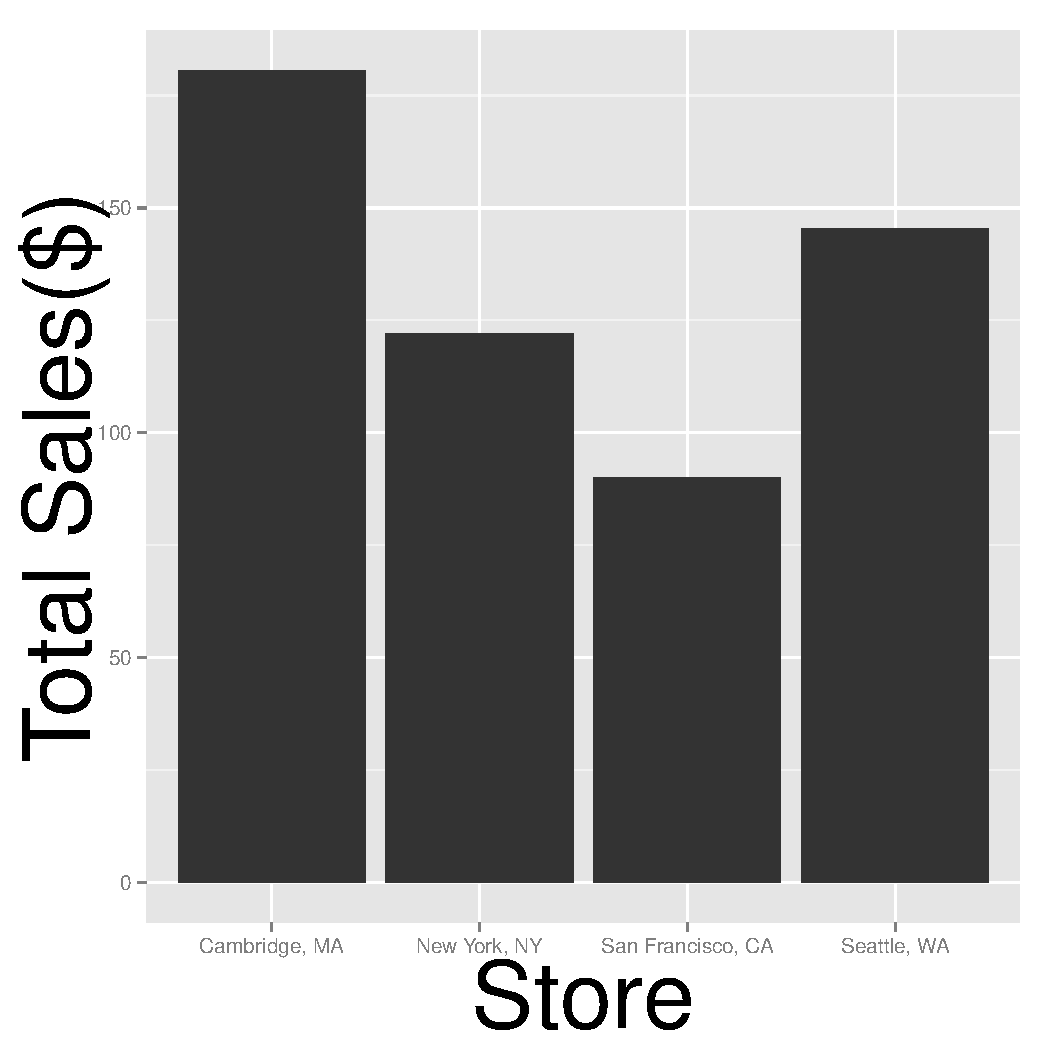
\includegraphics{Images/dist1.pdf}}}
  
}{%
  \caption{Visualization: Total \\ Sales by Store for
  Laserwave}\label{fig:staplerX}%
}
\end{floatrow}
\end{figure}

\begin{figure}
\CenterFloatBoxes
\begin{floatrow}
\ffigbox{%
  \hbox{\resizebox{2cm}{2cm}{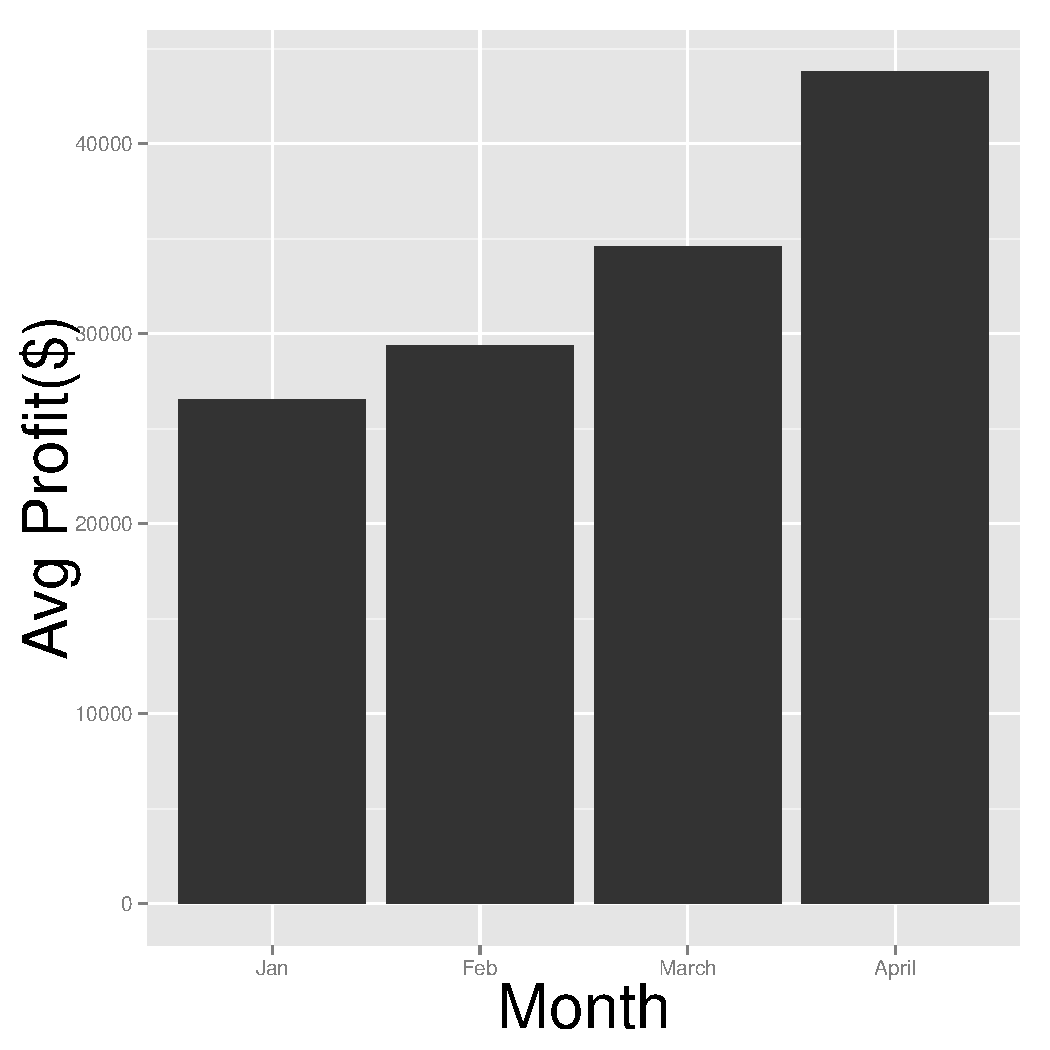
\includegraphics{Images/dist2.pdf}}}
  
}{%
  \caption{Scenario A: Total Sales by Store}\label{fig:staplerX-a}%
}
\killfloatstyle
\ffigbox{%
  \hbox{\resizebox{2cm}{2cm}{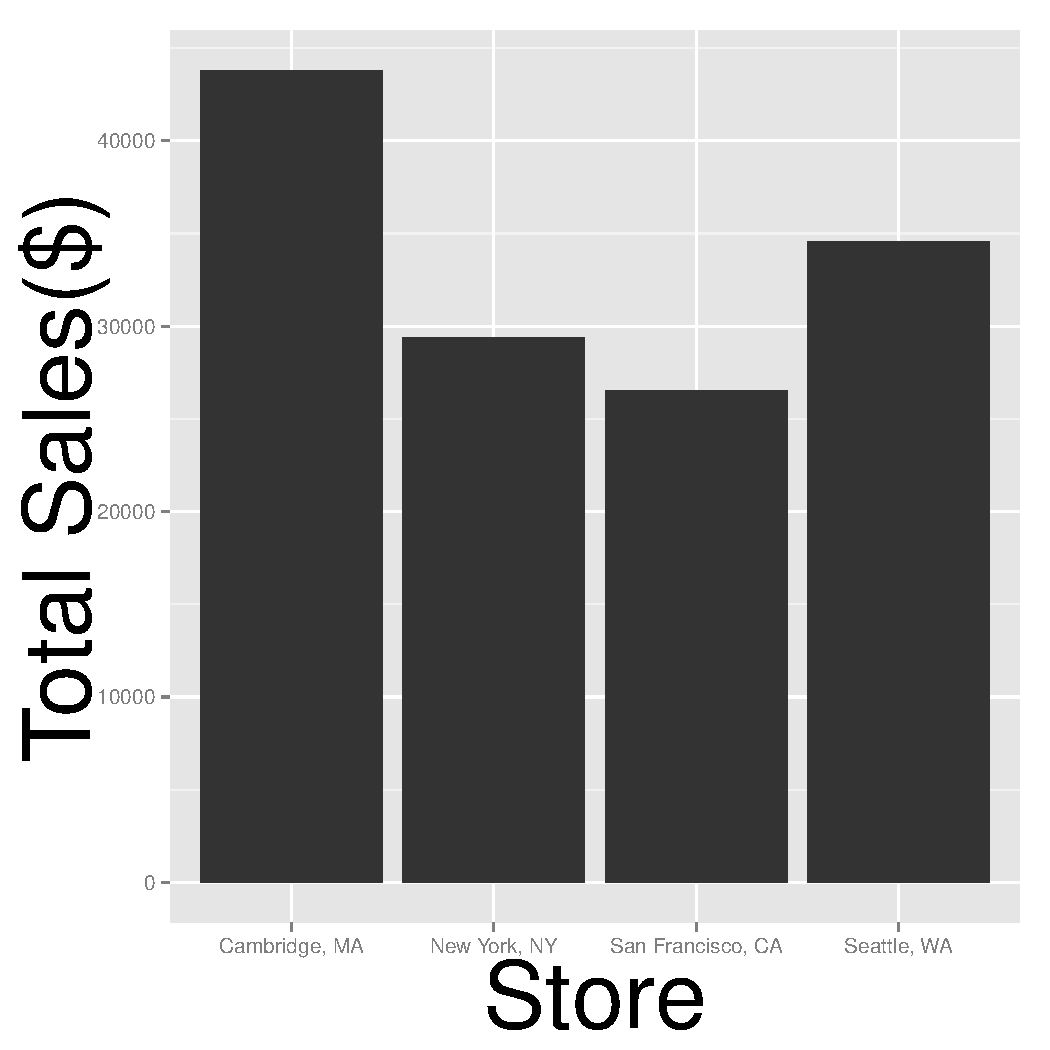
\includegraphics{Images/dist3.pdf}}}
  
}{%
  \caption{Scenario B: Total Sales by Store}\label{fig:staplerX-b}%
}
\end{floatrow}
\vspace{-10pt}
\end{figure}


% Since \SeeDB\ must rank views based on utility, accurately measuring 
% utility is cruicial. \SeeDB\ is based on the principle
% that it is the {\bf deviations from expected behavior that make a view
% interesting}. For instance, in the above example, the researcher would be
% interested in the fact that high-cost patients actually visit a specific set of
% doctors compared to the entire patient population. Similarly, the researcher
% would be interested in knowing that the high-cost patients have longer hospital
% stays compared to the rest of the population. Thus, given a query, interesting
% trends are those that differ significantly between the query and the underlying
% dataset. \SeeDB\ therefore assigns higher utility to views that show divergent
% trends. (Since it may be more appropriate to compare the high-cost patients with
% other patients having the same disease but lower cost, so \SeeDB\ allows the
% user to specify what dataset to compare with).


\stitle{Related Work:}
Over the past few years, the research community has introduced 
a number of interactive data analytics tools such as ShowMe, Polaris, and
Tableau~\cite{DBLP:journals/cacm/StolteTH08, DBLP:journals/tvcg/MackinlayHS07}
as well as tools like Profiler allow analysts to detect anomalies in data.
Unlike \SeeDB, which recommends visualizations automatically, the tools put the
onus on the analyst to specify the visualization to be generated.
Similar visualization specification tools have also been introduced
by the database community, including Fusion Tables~\cite{DBLP:conf/sigmod/GonzalezHJLMSSG10} 
and the Devise~\cite{DBLP:conf/sigmod/LivnyRBCDLMW97} toolkit.

There has been some work on browsing data cubes in OLAP, allowing
analysts to find explanations, get suggestions for next cubes to visit,
or identify generalizations or patterns starting from a single cube~\cite{DBLP:conf/vldb/Sarawagi99, 
DBLP:conf/vldb/SatheS01, DBLP:conf/vldb/Sarawagi00}. 
While we may be able to reuse the metrics from that line of work,
the same techniques will not apply directly to visualizations.



% \noindent There are several technical challenges that need to be addressed:
% 
% \begin{denselist}
% 
% \item For a given query, $n$, the total number of discriminating views, (even if
% we restrict ourselves to views that append a group-by and an aggregation) is
% likely to be very large to explore exhaustively and precisely. Generating each
% of $R_1(Q(D)),$  $\ldots,$ $R_n(Q(D))$, scoring them on utility, and then
% picking the best one is certainly not feasible for most databases. Thus, we need
% mechanisms to prune the space of views and compute their utility approximately.
% 
% \item Generating and scoring the discriminating views $R_i(Q(D))$ one-by-one may
% miss interesting optimization opportunities: First, we may share computation
% between discriminating views.  For example, the results of two views with
% different aggregates but the same group-by may be computed together in one
% query, followed by projecting out to reveal the two individual views.  Second,
% by evaluating the discriminating views in a deliberate order, we may be able to
% prune views with low utility (without evaluation) that are definitely not going
% to be recommended to the analyst.
% 
% \item Since visualizations tend to convey approximate information, e.g., a trend
% in a line plot may be more important than knowing the exact coordinates of each
% point, we can introduce approximations as part of \SeeDB.  Thus, the utility of
% a discriminating view may be computed approximately but efficiently, and the
% recommended discriminating views can be populated with approximate results,
% based on synopses of the base data or of the query result, that can be generated
% much more efficiently.
% 
% \end{denselist}
